\section{1}
\label{sect:A}
Description of section

\subsection{Subsection A}
Description of subsection a.
\begin{figure}[H]
  \centering
  \begin{subfigure}[b]{0.5\textwidth}
    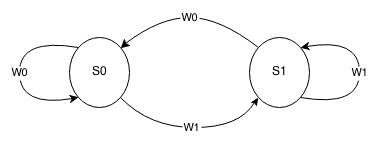
\includegraphics[width=\textwidth]{sd-gc}
    \caption{Test Figure 1}
    \label{fig:sd-gc}
  \end{subfigure}  
  
  \begin{subfigure}[b]{0.25\textwidth}
    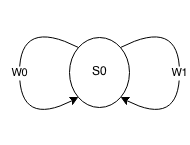
\includegraphics[width=\textwidth]{sd-sa0f}
    \caption{SA0 Fault}
    \label{fig:sd-sa0f}
  \end{subfigure}  
  \begin{subfigure}[b]{0.25\textwidth}
    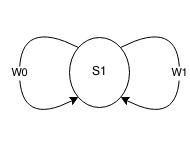
\includegraphics[width=\textwidth]{sd-sa1f}
    \caption{Test Figure 2}
    \label{fig:sd-sa1f}
  \end{subfigure}  

  \caption[Test Diagram]{Test Diagram \cite{VanDeGoor1991}}
  \label{fig:sd-sc}
\end{figure}

\subsection{subsection b}
Description of subsection b

Algorithms specify that the deleted neighborhood must be in the physical proximity of the base cell because only those cells are likely to influence the base cell.  Since the NPSF requires a specific pattern in memory which requires additional overhead, algorithms are written to detect all types of NPSF rather than a signle type.  Three classes of NPSF faults exist:
\begin{enumerate}
  \item Active NPSF (ANPSF) \cite{1675601}: the base cell's contents change due to changes in the pattern of the deleted neighborhood.
  \item Passive NPSF (PNPSF) \cite{1675601}: the base cell's contents cannot change due to specific pattern in the deleted neighborhood.
  \item Static NPSF (SNPSF) \cite{1676572}: the base cell's contents are forced to a specific value because of the contents of the deleted neighborhood
\end{enumerate}
